En aras de la simplicidad, supondremos que la función $f$ es solo una función de suma.

Dado un arreglo de enteros $A[0 \dots N-1]$. Un árbol de Fenwick es solo un arreglo $T[0 \dots N-1]$ 
, donde cada uno de sus elementos es igual a la suma de los elementos de $A$ en algún rango 
$[g(i),i]$:

$$T_i = \sum_{j = g(i)}^{i}{A_j},$$

dónde $g$ es alguna función que satisface $0 \le g(i) \le i$ que más adelante vamos a definir.

La estructura de datos se llama árbol, porque hay una buena representación de la estructura de datos como árbol, aunque no necesitamos modelar un árbol real con nodos y bordes. Solo necesitaremos mantener la matriz. $T$ para atender todas las consultas.

Ahora podemos escribir un pseudocódigo para las dos operaciones mencionadas anteriormente: obtener la suma de elementos de $A$ en el rango $[0, r]$ y actualizar (aumentar) algún elemento $A_i$ :
\begin{lstlisting}[language=C++]
def sum(int r):
   res = 0
   while (r >= 0):
      res += t[r]
      r = g(r) - 1
return res

def increase(int i, int delta):
   for all j with g(j) <= i <= j:
      t[j] += delta
\end{lstlisting}

La función \emph{sum} funciona de la siguiente manera:

\begin{enumerate}
	\item Primero, suma la suma del rango $[g(r), r]$ (es decir $T[r]$ ) en \emph{result}
	\item Luego salta al rango $[g(g(r)-1), g(r)-1]$ y adiciona la suma de este rango a \emph{result}
	\item Y asi sucesivamente salta en el rango de $[0, g(g( \dots g(r)-1\dots-1)-1)]$  hasta que llega al rango $[g(-1), -1]$ donde se detiene. En cada salto adiciona a \emph{result} el valor almacenado en el rango analizado. 
\end{enumerate}

La función \emph{increase} funciona de forma similar pero en dirección de incremento de los índices del rango:

\begin{enumerate}
	\item Sumas de rangos $[g(j),j]$ que satisfacen la condición $g(j)\le i \le j$ se incrementan 
	en delta, es decir $t[j]+= delta$. Por lo tanto, actualizamos todos los elementos en $T$ que 
	corresponden a rangos verdaderos de $A_i$.
\end{enumerate}


\subsection{\textbf{Definición de $g(i)$}}

El cómputo de $g(i)$ se define usando la siguiente operación simple: reemplazamos todos los $1$ bits en la representación binaria de $i$ con $0$. En otras palabras, si el dígito menos significativo de $i$ en binario es $0$, entonces $g(i)=i$. Y de lo contrario, el dígito menos significativo es un $1$, y tomamos esto $1$ y todos los demás que se arrastran $1$  y lo cambiamos a $0$. Por ejemplo, obtenemos:\\
\\
$g(11)=  g(1011_2)=  1000_2$\\
$g(12) = g(1100_2) = 1100_2$\\
$g(13) = g(1101_2) = 1100_2$\\
$g(14) = g(1110_2) = 1110_2$\\ 
$g(15) = g(1111_2) = 0000_2$

Existe una implementación simple que utiliza operaciones bit a bit para la operación no trivial descrita anteriormente:

$$g(i) = \quad i \quad \& \quad (i+1)$$

dónde $\&$ es el operador AND bit a bit. No es difícil convencerse de que esta solución hace lo 
mismo que la operación descrita anteriormente. Ahora, solo necesitamos encontrar una manera de 
iterar sobre todos $j$'s, tal que $g(j) \le i \le j$.


Es fácil ver que podemos encontrar todos esos $j$ es comenzando con $i$ y volteando el último bit 
no configurado. Llamaremos a esta operación $h(j)$ . por ejemplo, para $i = 10$ tenemos:\\

$10 = 0001010_2$\\
$h(10) = 11 = 0001011_2$\\
$h(11) = 15 = 0001111_2$\\
$h(15) = 31 = 0011111_2$\\
$h(31) = 63 = 0111111_2$\\
$\vdots$

Como era de esperar, también existe una forma sencilla de realizar $h$ usando operaciones bit a bit:

$$h(j) = j \quad | \quad (j+1) $$

dónde $|$ es el operador OR bit a bit.

La siguiente imagen muestra una posible interpretación del árbol de Fenwick como árbol. Los nodos del árbol muestran los rangos que cubren.

% TODO: \usepackage{graphicx} required
\begin{figure}[h!]
	\centering
	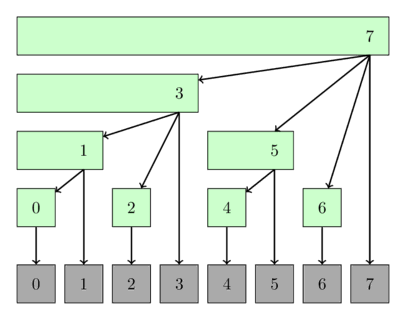
\includegraphics[width=0.5\linewidth]{img/binary_indexed_tree}
	\label{fig:binaryindexedtree}
\end{figure}

\subsection{Encontrar la suma en un arreglo}

El árbol de Fenwick normal solo puede responder consultas de suma del tipo $[0,r]$ usando sum(int 
r), sin embargo también podemos responder otras consultas del tipo $[l,r]$ calculando dos sumas 
$[0,r]$ y $[0,l-1]$ y restarlos. Esto se maneja en el metodo sum(int l, int r).

\subsection{Encontrar mínimo de $[0,r]$ en un arreglo}

Es obvio que no hay una manera fácil de encontrar el mínimo de rango $[l,r]$ usando el árbol de Fenwick, ya que el árbol de Fenwick solo puede responder consultas de tipo $[0,r]$. Además, cada vez que un valor es update'd, el nuevo valor tiene que ser menor que el valor actual. Ambas limitaciones significativas se deben a que la operación $min$ junto con el conjunto de números enteros no forma un grupo, ya que no hay elementos inversos.

\subsection{Enfoque de indexación basado en uno}

Para este enfoque, cambiamos los requisitos y la definición de $T[]$ y $g()$ un poco. Queremos $T[i]$ almacenar la suma de $[g(i)+1;i]$. Esto cambia un poco la implementación y permite una definición agradable similar para $g(i)$:

\begin{lstlisting}[language=C++]
def sum(int r):
   res = 0
   while (r > 0):
      res += t[r]
      r = g(r)
   return res

def increase(int i, int delta):
   for all j with g(j) < i <= j:
      t[j] += delta
\end{lstlisting}

El cómputo de $g(i)$ se define como: alternancia del último conjunto $1$ bit en la representación binaria de $i$.\\
$g(7) = g(111_2) = 110_2 = 6$ \\
$g(6) = g(110_2) = 100_2 = 4$ \\
$g(4) = g(100_2) = 000_2 = 0$ \\

El último bit establecido se puede extraer usando $i \quad \& \quad (-i)$, por lo que la operación se puede expresar como:


$$g(i) = i - (i \& (-i))$$

Y no es difícil ver que necesitas cambiar todos los valores $T[j]$ en la secuencia $i,h(i),h(h(i)), 
\dots$ cuando quieras actualizar $A[j]$ , dónde $h(i)$ Se define como:

$$h(i) = i + (i \& (-i))$$

Como puede ver, el principal beneficio de este enfoque es que las operaciones binarias se complementan muy bien

\subsection{Operaciones de rango}

Un árbol Fenwick puede admitir las siguientes operaciones de rango:

\begin{enumerate}
	\item \textbf{Actualización de puntos y consulta de rango:} Este es solo el árbol Fenwick ordinario como se explicó anteriormente.
	\item \textbf{Actualización de rango y consulta de posición:} Usando trucos simples, también 
	podemos hacer las operaciones inversas: aumentar rangos y consultar valores únicos. Deje que el 
	árbol de Fenwick se inicialice con ceros. Supongamos que queremos incrementar el intervalo$[l, r]$ por $x$. Realizamos operaciones de actualización de dos puntos en el árbol de Fenwick, que son add(l,x) y add(r+1, -x). Si queremos obtener el valor de $A[i]$ , solo necesitamos tomar la suma del prefijo usando el método de suma de rango ordinario. Para ver por qué esto es cierto, podemos centrarnos de nuevo en la operación de incremento anterior. Si $i<l$ , entonces las dos operaciones de actualización no tienen efecto en la consulta y obtenemos la suma $0$ . Si $i\in[l,r]$, entonces obtenemos la respuesta $x$ debido a la primera operación de actualización. Y si $i>r$, entonces la segunda operación de actualización cancelará el efecto de la primera.
	\item \textbf{Actualización de rango y consulta de rango:} Para admitir tanto las actualizaciones de rango como las consultas de rango, utilizaremos dos BIT, a saber $B_1[]$ y $B_2[]$, inicializado con ceros. Supongamos que queremos incrementar el intervalo $[l,r]$ por el valor $x$. De manera similar al método anterior, realizamos actualizaciones de dos puntos en $B_1$: add(B1,l,x)y add(B1,r+1,-x). Y también actualizamos $B_2$. Los detalles se explicarán más adelante.

\begin{lstlisting}[language=C++]	
def range_add(l, r, x):
   add(B1, l, x)
   add(B1, r+1, -x)
   add(B2, l, x*(l-1))
   add(B2, r+1, -x*r))
\end{lstlisting}	

Después de la actualización de rango $(l, r, x)$ la consulta de suma de rango debe devolver los siguientes valores: 
% TODO: \usepackage{graphicx} required
\begin{figure}[h!]
	\centering
	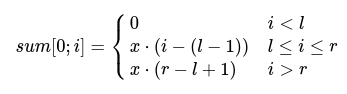
\includegraphics[width=0.35\linewidth]{img/binary_indexed_tree_1}
	\label{fig:binaryindexedtree1}
\end{figure}

Podemos escribir la suma del rango como diferencia de dos términos, donde usamos $B_1$ para el primer término y $B_2$ para segundo término. La diferencia de las consultas nos dará el \emph{prefix\_sum} sobre $[0,i]$.

\begin{figure}[h!]
	\centering
	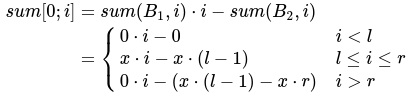
\includegraphics[width=0.35\linewidth]{img/binary_indexed_tree_2}
	\label{fig:binaryindexedtree2}
\end{figure}

La última expresión es exactamente igual a los términos requeridos. Así podemos usar $B_2$ para eliminar términos adicionales cuando multiplicamos $B_1[i]\times i$ .

Podemos encontrar sumas de rangos arbitrarias al calcular las sumas de prefijos para $l-1$ y $r$ y tomando la diferencia de ellos de nuevo.

\begin{lstlisting}[language=C++]	
def add(b, idx, x):
   while idx<=N:
      b[idx]+=x
      idx+=idx&-idx

def range_add(l,r,x):
   add(B1,l,x)
   add(B1,r+1,-x)
   add(B2,l,x*(l-1))
   add(B2,r+1,-x*r)

def sum(b, idx):
   total=0
   while idx>0:
      total+=b[idx]
      idx-=idx&-idx
   return total

def prefix_sum(idx):
   return sum(B1,idx)*idx-sum(B2,idx)

def range_sum(l, r):
return sum(r) - sum(l-1)
\end{lstlisting}

\end{enumerate}




